\section{Further Examples of Metric Spaces}

The $l^p$ proof is a bit annoying, I had to read through it carefully to really get it.

We have $p \in \R$, and $x = (\xi_j) = (\xi_1, \xi_2, \dots)$ such that

\begin{equation}
  \sum_{j=1}^\infty |\xi_j|^p < \infty. \tag{$p\geq 1$}
\end{equation}

and the metric is defined by

\begin{equation}
  d(x, y) = \pa{\sum_{j=1}^\infty |\xi_j - \eta_j|^p}^{1/p}.
\end{equation}

For $p= 2$, we have the Hilbert space $l^2$.

We now want to prove that $l^p$ is a metric space.

\begin{proof}
  Properties 1-3 are pretty straightforward, so we really just need to show convergence and the triangle inequality.

  We are starting with a auxiliary inequality
  \begin{equation}
    \frac{1}{p} + \frac{1}{q} = 1
  \end{equation}

  From this inequality, where $p, q$ are \textbf{conjugate exponents}, we can derive $1/(p-1) = q - 1$. Therefore, we can say
  \begin{equation}
    u = t^{p-1} \implies t = u^{1/(p-1)} = u^{q-1}.
  \end{equation}

  Now, suppose $\alpha, \beta \geq 0$. Since $\alpha\beta$ is the area of a rectangle in \ref{fig:youngs_inequality}, we can bound it above by the integral curves.
  The intuition here is, we want to consider the area under the curve, vertically and horizontally. We have 3 cases:
  \begin{enumerate}
    \item If the corner $(\alpha, \beta)$ is exactly at the corner of the rectangle, then the rectangle area is exactly the sum of the two areas.
    \item If the end of the curve at $\alpha$ is above $\beta$, then the rectangle is smaller than the sum of the two areas, because the curve has more area above the $\beta$ line.
    \item If the end of the curve at $\alpha$ is below $\beta$, then the rectangle is still smaller than the sum of the two areas, since it has more horizontal area past $\alpha$.
  \end{enumerate}

  \begin{figure}[H]
    \centering
    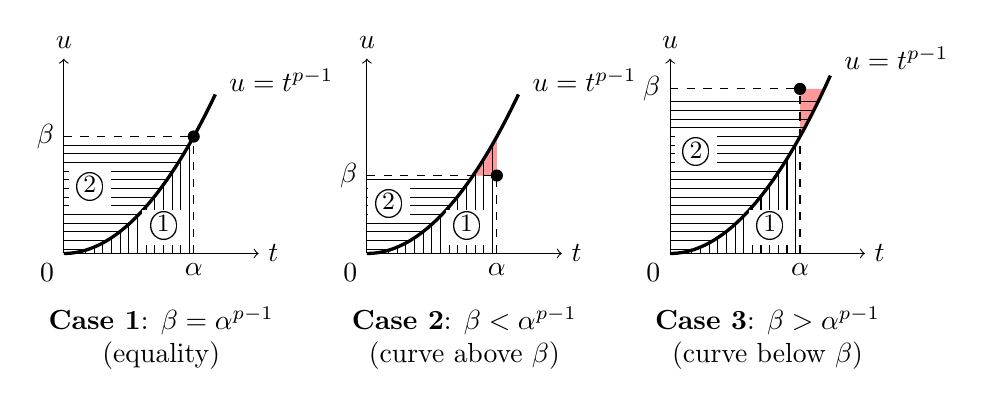
\begin{tikzpicture}[scale=0.55]
      % Case 1: Equality - corner exactly on curve
      \begin{scope}
        % Axes
        \draw[->] (0,0) -- (4.5,0) node[right] {$t$};
        \draw[->] (0,0) -- (0,4.5) node[above] {$u$};
        \node[below left] at (0,0) {$0$};

        % For equality: beta = alpha^{p-1} (corner on curve)
        \def\alph{3}
        \pgfmathsetmacro{\bet}{0.3*\alph*\alph} % beta = 2.7

        % Region 1 - vertical lines (area under curve from 0 to alpha)
        \foreach \x in {0.1,0.3,...,2.9} {
          \pgfmathsetmacro{\yval}{0.3*\x*\x}
          \draw[thin] (\x,0) -- (\x,\yval);
        }

        % Region 2 - horizontal lines (area to left of curve from 0 to beta)
        \foreach \y in {0.1,0.3,...,2.5} {
          \pgfmathsetmacro{\xval}{sqrt(\y/0.3)}
          \draw[thin] (0,\y) -- (\xval,\y);
        }

        % The curve u = t^{p-1}
        \draw[very thick, domain=0:3.5, samples=100] plot (\x, {0.3*\x*\x});

        % Rectangle boundary - corner ON the curve
        \draw[dashed] (\alph,0) -- (\alph,\bet);
        \draw[dashed] (0,\bet) -- (\alph,\bet);
        \fill (\alph,\bet) circle (4pt); % Mark the corner point

        % Labels
        \node[below] at (\alph,0) {$\alpha$};
        \node[left] at (0,\bet) {$\beta$};
        \node[fill=white, inner sep=2pt] at (2.3,0.6) {\textcircled{\small 1}};
        \node[fill=white, inner sep=2pt] at (0.6,1.5) {\textcircled{\small 2}};
        \node[right] at (3.6,4) {$u = t^{p-1}$};
        \node[below, align=center] at (2.25,-1) {\textbf{Case 1}: $\beta = \alpha^{p-1}$\\(equality)};
      \end{scope}

      % Case 2: Curve at alpha is ABOVE beta
      \begin{scope}[xshift=7cm]
        % Axes
        \draw[->] (0,0) -- (4.5,0) node[right] {$t$};
        \draw[->] (0,0) -- (0,4.5) node[above] {$u$};
        \node[below left] at (0,0) {$0$};

        % beta < alpha^{p-1} (curve goes above beta at alpha)
        \def\alph{3}
        \def\bet{1.8} % Below curve value of 2.7
        \pgfmathsetmacro{\curveatalpha}{0.3*\alph*\alph}

        % Extra sliver in RED - area between beta and curve (above rectangle)
        \fill[red!40] plot[domain={sqrt(\bet/0.3)}:\alph, samples=50] (\x, {0.3*\x*\x}) -- (\alph,\bet) -- ({sqrt(\bet/0.3)},\bet) -- cycle;

        % Region 1 - vertical lines (area under curve from 0 to alpha)
        \foreach \x in {0.1,0.3,...,2.9} {
          \pgfmathsetmacro{\yval}{0.3*\x*\x}
          \draw[thin] (\x,0) -- (\x,\yval);
        }

        % Region 2 - horizontal lines (area to left of curve from 0 to beta)
        \foreach \y in {0.1,0.3,...,1.7} {
          \pgfmathsetmacro{\xval}{sqrt(\y/0.3)}
          \draw[thin] (0,\y) -- (\xval,\y);
        }

        % The curve u = t^{p-1}
        \draw[very thick, domain=0:3.5, samples=100] plot (\x, {0.3*\x*\x});

        % Rectangle boundary - corner BELOW the curve
        \draw[dashed] (\alph,0) -- (\alph,\bet);
        \draw[dashed] (0,\bet) -- (\alph,\bet);
        \fill (\alph,\bet) circle (4pt); % Mark the corner point

        % Labels
        \node[below] at (\alph,0) {$\alpha$};
        \node[left] at (0,\bet) {$\beta$};
        \node[fill=white, inner sep=2pt] at (2.3,0.6) {\textcircled{\small 1}};
        \node[fill=white, inner sep=2pt] at (0.5,1.1) {\textcircled{\small 2}};
        \node[right] at (3.6,4) {$u = t^{p-1}$};
        \node[below, align=center] at (2.25,-1) {\textbf{Case 2}: $\beta < \alpha^{p-1}$\\(curve above $\beta$)};
      \end{scope}

      % Case 3: Curve at alpha is BELOW beta
      \begin{scope}[xshift=14cm]
        % Axes
        \draw[->] (0,0) -- (4.5,0) node[right] {$t$};
        \draw[->] (0,0) -- (0,4.5) node[above] {$u$};
        \node[below left] at (0,0) {$0$};

        % beta > alpha^{p-1} (curve goes below beta at alpha)
        \def\alph{3}
        \def\bet{3.8} % Above curve value of 2.7
        \pgfmathsetmacro{\curveatalpha}{0.3*\alph*\alph}

        % Extra sliver in RED - area between alpha and curve (past rectangle horizontally)
        \fill[red!40] plot[domain=\alph:{sqrt(\bet/0.3)}, samples=50] (\x, {0.3*\x*\x}) -- ({sqrt(\bet/0.3)},\bet) -- (\alph,\bet) -- (\alph,\curveatalpha) -- cycle;

        % Region 1 - vertical lines (area under curve from 0 to alpha)
        \foreach \x in {0.1,0.3,...,2.9} {
          \pgfmathsetmacro{\yval}{0.3*\x*\x}
          \draw[thin] (\x,0) -- (\x,\yval);
        }

        % Region 2 - horizontal lines (area to left of curve from 0 to beta)
        \foreach \y in {0.1,0.3,...,3.6} {
          \pgfmathsetmacro{\xval}{sqrt(\y/0.3)}
          \draw[thin] (0,\y) -- (\xval,\y);
        }

        % The curve u = t^{p-1}
        \draw[very thick, domain=0:3.7, samples=100] plot (\x, {0.3*\x*\x});

        % Rectangle boundary - corner ABOVE the curve
        \draw[dashed] (\alph,0) -- (\alph,\bet);
        \draw[dashed] (0,\bet) -- (\alph,\bet);
        \fill (\alph,\bet) circle (4pt); % Mark the corner point

        % Labels
        \node[below] at (\alph,0) {$\alpha$};
        \node[left] at (0,\bet) {$\beta$};
        \node[fill=white, inner sep=2pt] at (2.3,0.6) {\textcircled{\small 1}};
        \node[fill=white, inner sep=2pt] at (0.6,2.3) {\textcircled{\small 2}};
        \node[right] at (3.8,4.5) {$u = t^{p-1}$};
        \node[below, align=center] at (2.25,-1) {\textbf{Case 3}: $\beta > \alpha^{p-1}$\\(curve below $\beta$)};
      \end{scope}
    \end{tikzpicture}
    \caption{Integral inequality cases. The red areas are the excess}
    \label{fig:youngs_inequality}
  \end{figure}

  The diagrams in \ref{fig:youngs_inequality} illustrate these cases. Now, we can derive

  \begin{equation}
    \alpha\beta \leq \int_0^\alpha t^{p-1} \dd{t} + \int_0^\beta u^{q-1} \dd{u} = \frac{\alpha^p}{p} + \frac{\beta^q}{q}.
    \label{eq:youngs_inequality}
  \end{equation}

  Now, suppose we have sequences $(\xi_j), (\eta_j)$, such that
  \begin{equation}
    \sum_{j=1}^\infty |\xi_j|^p = 1, \quad \sum_{j=1}^\infty |\eta_j|^q = 1.
  \end{equation}
  From \eqref{eq:youngs_inequality}, and summing over $j$, we have
  \begin{equation}
    \sum_{j=1}^\infty |\xi_j \eta_j| \leq \sum_{j=1}^\infty \pa{\frac{|\xi_j|^p}{p} + \frac{|\eta_j|^q}{q}} =
    \frac{1}{p} + \frac{1}{q} = 1.
    \label{eq:normalized_holder}
  \end{equation}
  Now, if we want to choose any arbitrary sequences $(\xi_j), (\eta_j)$, we can normalize them by defining
  \begin{equation}
    \tilde{\xi_j} = \frac{\xi_j}{\pa{\sum_{k=1}^\infty |\xi_k|^p}^{1/p}},
    \quad \tilde{\eta_j} = \frac{\eta_j}{\pa{\sum_{k=1}^\infty |\eta_k|^q}^{1/q}},
  \end{equation}
  and we can now substitute into \eqref{eq:normalized_holder} to get
  \begin{align*}
    \sum_{j=1}^\infty |\xi_j \eta_j| &\leq 1\\
    \sum_{j=1}^\infty \abs{
      \frac{\xi_j}{\pa{\sum_{k=1}^\infty |\xi_k|^p}^{1/p}} \cdot
      \frac{\eta_j}{\pa{\sum_{k=1}^\infty |\eta_k|^q}^{1/q}}
    } &\leq 1 \tag{Substitute normalizations}\\
    \sum_{j=1}^\infty |\xi_j \eta_j| &\leq
    \pa{\sum_{k=1}^\infty |\xi_k|^p}^{1/p}
    \pa{\sum_{k=1}^\infty |\eta_k|^q}^{1/q}.
  \end{align*}
  This now gives us \textbf{Hölder's inequality}.

  We now need to prove \textbf{Minkoswki's inequality}, which is the triangle inequality for $l^p$.
  We start by using $\omega_j = \xi_j + \eta_j$. Then, what we can do is use the triangle inequality to get
  \begin{align*}
    \abs{\omega_j} &\leq \abs{\xi_j + \eta_j}\\
    \abs{\omega_j}^p &\leq \abs{\xi_j + \eta_j}\abs{\omega_j}^{p-1} \\
    \abs{\omega_j}^p &\leq \pa{\abs{\xi_j} + \abs{\eta_j}}\abs{\omega_j}^{p-1} \tag{Triangle inequality}\\
    \sum\abs{\omega_j}^p &\leq \sum \abs{\xi_j}\abs{\omega_j}^{p-1} + \sum\abs{\eta_j}\abs{\omega_j}^{p-1} \tag{Applying sum}\\
  \end{align*}
  Now we can apply Hölder's inequality to each of the sums on the right-hand side, where we have conjugate exponents $p$ and $q$, which gives us:
  \begin{align*}
    \sum\abs{\omega_j}^p
    &\leq
    \pa{
      \sum \abs{\xi_j}^p
    }^{1/p}
    \pa{
      \sum \abs{\omega_j}^{(p-1)q}
    }^{1/q}
    +
    \pa{
      \sum \abs{\eta_j}^p
    }^{1/p}
    \pa{
      \sum \abs{\omega_j}^{(p-1)q}
    }^{1/q}\\
    &\leq
    \pa{
      \sum \abs{\xi_j}^p
    }^{1/p}
    \pa{
      \sum \abs{\omega_j}^p
    }^{1/q}
    +
    \pa{
      \sum \abs{\eta_j}^p
    }^{1/p}
    \pa{
      \sum \abs{\omega_j}^p
    }^{1/q} \tag{Since $(p-1)q = p$}\\
    &\leq
    \pbra{
      \pa{
        \sum \abs{\xi_j}^p
      }^{1/p}
      +
      \pa{
        \sum \abs{\eta_j}^p
      }^{1/p}
    }
    \pa{
      \sum \abs{\omega_j}^p
    }^{1/q}
  \end{align*}
  Finally, dividing both sides by $\pa{\sum \abs{\omega_j}^p}^{1/q}$:
  \begin{align*}
    \pa{\sum \abs{\omega_j}^p}^{1 - 1/q}
    &\leq
    \pa{\sum \abs{\xi_j}^p}^{1/p}
    +
    \pa{\sum \abs{\eta_j}^p}^{1/p}
  \end{align*}
  Since $1 - \frac{1}{q} = \frac{1}{p}$ (from $\frac{1}{p} + \frac{1}{q} = 1$), we have
  \begin{equation}
    \pa{\sum \abs{\xi_j + \eta_j}^p}^{1/p}
    \leq
    \pa{\sum \abs{\xi_j}^p}^{1/p}
    +
    \pa{\sum \abs{\eta_j}^p}^{1/p}
  \end{equation}
  which is \textbf{Minkowski's inequality}.

  Finally, we need to show the triangle inequality for the metric.

  We take $x = (\xi_j), y = (\eta_j), z = (\zeta_j)$, and we have
  \begin{align*}
    d(x, z) &= \pa{\sum |\xi_j - \zeta_j|^p}^{1/p} \\
    &= \pa{\sum |\xi_j - \eta_j + \eta_j - \zeta_j|^p}^{1/p} \\
    &\leq \pa{\sum |\xi_j - \eta_j|^p}^{1/p} + \pa{\sum |\eta_j - \zeta_j|^p}^{1/p} \tag{Minkowski's inequality}\\
    &= d(x, y) + d(y, z).
  \end{align*}
  This completes the proof that $l^p$ is a metric space.
\end{proof}

\bx{
  if we have $\mu_j$ such that $\sum \mu_j$ converges instead of $1/2^j$, then we just need to show
  \begin{equation*}
    d(x, y) = \sum_{j=1}^\infty \mu_j \frac{|\xi_j - \eta_j|}{1 + |\xi_j - \eta_j|}
  \end{equation*}
  is a metric. The properties 1-3 are easy, we just need to show convergence. But this is easy since $    \frac{|\xi_j - \eta_j|}{1 + |\xi_j - \eta_j|} \leq 1$, so we have
  \begin{equation*}
    d(x, y) \leq \sum_{j=1}^\infty \mu_j,
  \end{equation*}
  which converges by assumption.
}

\bx{
  Suppose we have $\alpha, \beta > 0$. Then from \eqref{eq:youngs_inequality}, we have
  \begin{equation*}
    \alpha\beta \leq \frac{\alpha^p}{p} + \frac{\beta^q}{q}.
  \end{equation*}
  If we plug in $p = q = 2$, we have
  \begin{align*}
    \alpha\beta &\leq \frac{\alpha^2}{2} + \frac{\beta^2}{2} \\
    \frac{\alpha\beta}{2} &\leq \frac{\alpha^2 + \beta^2}{4} \\
    \alpha\beta &\leq \frac{\alpha^2 + 2\alpha\beta + \beta^2}{4} \\
    \sqrt{\alpha\beta} &\leq \frac{\alpha + \beta}{2}.
  \end{align*}
}

\bx{
  Let's start with the Cauchy-Schwarz inequality for sums:
  \begin{equation*}
    \sum_{j=1}^{n} \abs{\xi_j \eta_j}
    \leq
    \sqrt{\sum_{k=1}^{n} \abs{\xi_k}^2}
    \sqrt{\sum_{m=1}^{n} \abs{\eta_m}^2}
  \end{equation*}
  Now, choose
  \begin{equation}
    \eta_j =
    \begin{cases}
      1 & j = 1, 2, \dots, n\\
      0 & \text{otherwise}
    \end{cases}
  \end{equation}
  Then, if we square both sides of the inequality, we get
  \begin{equation*}
    \pa{\sum_{j=1}^{n} \abs{\xi_j}}^2
    \leq
    n
    \sum_{k=1}^{n} \abs{\xi_k}^2.
  \end{equation*}
}

\bx{
  Consider the sequence $\xi_n = \frac{1}{\log(n+1)}$.

  \textbf{Converges to 0:} Since $\log(n+1) \to \infty$ as $n \to \infty$, we have $\xi_n \to 0$.

  \textbf{Not in any $l^{p}$:} For any $p \geq 1$, we show that
  \[
    \sum_{n=1}^{\infty} \abs{\xi_n}^p = \sum_{n=1}^{\infty} \frac{1}{(\log(n+1))^p} = \infty.
  \]
  Since $\log(n+1)$ grows slower than any positive power of $n$, for large $n$ we have
  \[
    \frac{1}{(\log(n+1))^p} > \frac{1}{n}
  \]
  and the harmonic series $\sum 1/n$ diverges. By comparison, $\sum \frac{1}{(\log(n+1))^p}$ diverges for all $p \geq 1$.

  Therefore $(\xi_n) = \left(\frac{1}{\log(n+1)}\right)$ converges to 0 but is not in any $l{p}$ space.
}

\bx{
  Consider the sequence $\xi_n = \frac{1}{n}$.

  \textbf{In $l^{p}$ for $p > 1$:}
  \[
    \sum_{n=1}^{\infty} \abs{\xi_n}^p = \sum_{n=1}^{\infty} \frac{1}{n^p} < \infty
  \]
  since the $p$-series converges for $p > 1$.

  \textbf{Not in $l^{1}$:}
  \[
    \sum_{n=1}^{\infty} \abs{\xi_n} = \sum_{n=1}^{\infty} \frac{1}{n} = \infty
  \]
  since the harmonic series diverges.
}

\bx{
  AFSOC $A \subset B$ and $\delta(A) > \delta(B)$.

  Then, $\exists x, y \in A$ such that $d(x, y) > d(x', y')$ for all $x', y' \in B$.
  But this is a contradition, since $A \subset B$, so all $x, y \in A$ are also in $B$.
  Therefore, we must have $\delta(A) \leq \delta(B)$.
}

\bx{
  If $\delta(A) = 0$, then $\forall x, y \in A$, we have $d(x, y) = 0$. By property 2 of metric spaces, this implies $x = y$, so $A$ contains a single point.

  Suppose $A$ contains a single point, then $\forall x, y \in A$, we have $x = y$, so $d(x, y) = 0$. Thus, $\delta(A) = 0$.
}

\bx{
  To explain $D$ in plain English, it is the minimum distance of two points coming from two sets $A, B$.
  Now, the question is, does $D$ define a metric on the power set of $X$?

  We see that, property 2 is violated, because as long as $A$ and $B$ share a common point, we have $D(A, B) = 0$, but $A$ and $B$ could be different sets.
}

\bx{
  The $\emptyset$ in the text looks like $\phi$ (phi). Anyways, if $A\cap B \neq \emptyset$, then $\exists x \in A \cap B$.
  This means that $\exists x \in A, \in B$, so $d(x, x) = 0$, so $D(A, B) = 0$.

  Now the converse, if $D(A, B) = 0$, then $\inf\{d(x, y) : x \in A, y \in B\} = 0$.
  Suppose $A \cap B = \emptyset$, then $d(x, y) > 0$.
  But we can choose $\epsilon = d(x, y)/2$, which leads to a contradiction.
  Thus, we must have $A \cap B \neq \emptyset$
}

\bx{
  For any $x, y \in X$, $b \in B$, we have from the triangle inequality that
  \begin{align*}
    d(x, b) &\leq d(x, y) + d(y, b)
  \end{align*}
  Taking the infimum over $b \in B$ on both sides:
  \begin{align*}
    \inf_{b \in B} d(x, b) &\leq \inf_{b \in B} \pbra{d(x, y) + d(y, b)}
  \end{align*}
  Since $d(x, y)$ does not depend on $b$, we can pull it out of the infimum:
  \begin{align*}
    D(x, B) &\leq d(x, y) + \inf_{b \in B} d(y, b) = d(x, y) + D(y, B)
  \end{align*}
  Therefore $D(x, B) - D(y, B) \leq d(x, y)$.

  Now, applying the same argument but starting with $d(y, b) \leq d(y, x) + d(x, b)$:
  \begin{align*}
    D(y, B) &\leq d(y, x) + D(x, B) = d(x, y) + D(x, B)
  \end{align*}
  Therefore $D(y, B) - D(x, B) \leq d(x, y)$.

  Combining both inequalities:
  \begin{equation*}
    \abs{D(x, B) - D(y, B)} \leq d(x, y)
  \end{equation*}
}

\bx{
  We want to show that
  \begin{equation}
    \tilde{d}(x, y) = \frac{d(x, y)}{1 + d(x, y)}
  \end{equation}
  is still a metric.

  Let's walk through the four properties:
  \begin{enumerate}
    \item Since $d(x, y) \geq 0$, we have $\tilde{d}(x, y) \geq 0$. It is real valued because $d$ is, and it's finite because $d$ is finite, and $\tilde{d}(x, y)$ is bounded by $(0, 1)$.
    \item If $\tilde{d}(x, y) = 0$, then $d(x, y) = 0$, which implies $x = y$. Conversely, if $x = y$, then $d(x, y) = 0$, so $\tilde{d}(x, y) = 0$.
    \item $\tilde{d}(x, y) = \frac{d(x, y)}{1 + d(x, y)} = \frac{d(y, x)}{1 + d(y, x)} = \tilde{d}(y, x)$.
    \item For the triangle inequality, we can show
      \begin{align*}
        \tilde{d}(x, z) &= \frac{d(x, z)}{1 + d(x, z)} \\
        &\leq \frac{
          d(x, y) + d(y, z)
        }{
          1 + d(x, y) + d(y, z)
        } \tag{By triangle inequality}\\
        &\leq \frac{
          d(x, y)
        }{
          1 + d(x, y) + d(y, z)
        }
        + \frac{
          d(y, z)
        }{
          1 + d(x, y) + d(y, z)
        } \\
        &\leq \frac{
          d(x, y)
        }{
          1 + d(x, y)
        }
        + \frac{
          d(y, z)
        }{
          1 + d(y, z)
        } \tag{Since $d(x, y), d(y, z) \geq 0$, this makes the denom smaller, thus the fraction bigger}\\
        &\leq \tilde{d}(x, y) + \tilde{d}(y, z)
      \end{align*}
  \end{enumerate}
}

\bx{
  Since $A, B$ are bounded sets, we know $\exists p_A, p_B$ such that $\forall x \in A, y \in B$, $\exists M_A, M_B \in \mathbb{R}$ such that
  \begin{equation*}
    d(x, p_A) \leq M_A, \quad d(y, p_B) \leq M_B.
  \end{equation*}

  Let's choose $p_A$ to be our anchor point. Then, for any $p \in A \cup B$, we have two cases
  \begin{enumerate}
    \item $p \in A$, then $d(p, p_A) \leq M_A$ by definition.
    \item $p \in B$, then we can do:
      \begin{align*}
        d(p, p_A) &\leq d(p, p_B) + d(p_B, p_A) \tag{Triangle inequality}\\
        &\leq M_B + d(p_B, p_A) \tag{Since $p \in B$}\\
        &\leq M_B + K
      \end{align*}
      where $K = d(p_B, p_A)$ is a constant, and this is true because $d$ is a metric and is finite and real-valued, and $p_B, p_A \in X$ (the overall metric space).
  \end{enumerate}
  Therefore, we can bound $A \cup B$ by $\max(M_A, M_B + K)$, so $A \cup B$ is bounded.
}

\bx{
  We have the metric for the $X = X_1 \times X_2$ space defined as
  \begin{equation*}
    d(x, y) = d_1(x_1, y_1) + d_2(x_2, y_2).
  \end{equation*}
  We want to show that this is a metric.
  \begin{enumerate}
    \item Real, $\geq 0$, finite, follows from $d_1, d_2$ are both real-valued and non-negative and finite.
    \item $d(x, y) = 0$ implies $d_1(x_1, y_1) + d_2(x_2, y_2) = 0$. Since both $d_1, d_2 \geq 0$, we must have $d_1(x_1, y_1) = 0$ and $d_2(x_2, y_2) = 0$, which implies $x_1 = y_1$ and $x_2 = y_2$, so $x = y$. Conversely, if $x = y$, then $d(x, y) = d_1(x_1, y_1) + d_2(x_2, y_2) = 0$.
    \item Symmetry follows from the symmetry of $d_1, d_2$:
      \begin{align*}
        d(x, y) &= d_1(x_1, y_1) + d_2(x_2, y_2) \\
        &= d_1(y_1, x_1) + d_2(y_2, x_2) \\
        &= d(y, x).
      \end{align*}
    \item Triangle inequality:
      \begin{align*}
        d(x, z) &= d_1(x_1, z_1) + d_2(x_2, z_2) \\
        &\leq d_1(x_1, y_1) + d_1(y_1, z_1) + d_2(x_2, y_2) + d_2(y_2, z_2) \tag{Triangle inequality for $d_1, d_2$}\\
        &= d(x, y) + d(y, z).
      \end{align*}
  \end{enumerate}
}

\bx{
  We want to show the same as the previous exercise, except for the metric defined as
  \begin{equation*}
    d(x, y) = \sqrt{d_1(x_1, y_1)^2 + d_2(x_2, y_2)^2}.
  \end{equation*}
  The first three properties are straightforward from the properties of $d_1, d_2$.
  For the triangle inequality, we can use Minkowski's inequality:
  \begin{align*}
    d(x, z) &= \sqrt{d_1(x_1, z_1)^2 + d_2(x_2, z_2)^2} \\
    &\leq \sqrt{\pa{d_1(x_1, y_1) + d_1(y_1, z_1)}^2 + \pa{d_2(x_2, y_2) + d_2(y_2, z_2)}^2} \tag{Triangle inequality for $d_1, d_2$}\\
    &\leq \sqrt{d_1(x_1, y_1)^2 + d_2(x_2, y_2)^2} + \sqrt{d_1(y_1, z_1)^2 + d_2(y_2, z_2)^2} \tag{Minkowski's inequality}\\
    &= d(x, y) + d(y, z).
  \end{align*}
}

\bx{
  We want to show the metric space defined by
  \begin{equation*}
    d(x, y) = \max\pa{d_1(x_1, y_1), d_2(x_2, y_2)}
  \end{equation*}
  is a metric. The first three properties are straightforward from the properties of $d_1, d_2$.
  For the triangle inequality, we have
  \begin{align*}
    d(x, z) &= \max\pa{d_1(x_1, z_1), d_2(x_2, z_2)} \\
    &\leq \max\pa{d_1(x_1, y_1) + d_1(y_1, z_1), d_2(x_2, y_2) + d_2(y_2, z_2)} \tag{Triangle inequality for $d_1, d_2$}\\
    &\leq \max\pa{d_1(x_1, y_1), d_2(x_2, y_2)} + \max\pa{d_1(y_1, z_1), d_2(y_2, z_2)} \tag{Properties of max}\\
    &= d(x, y) + d(y, z).
  \end{align*}
}